%Teorema dell'arco sicuro va spostato in avanti
\chapter{Minimum Spanning Tree - MST}
\section{Teorema dell'arco sicuro}
Dati un grafo connesso non orientato e pesato $G=(V,E)$, un sottoinsieme A dell'insieme T di archi di un
Minimum Spanning Tree (MST) e un qualsiasi taglio che rispetti A, allora un arco leggero (u,v) del taglio è
sicuro per A, cioè $A \cup \{(u,v)\} \subseteq T$.
\subsection{Proof}
Considero T \ra insieme di archi di un MST.\\
$A \subseteq T \rt$ sottoinsieme di T.\\
Taglio che rispetta A = (\tikz \fill[green] (0,0) circle (2pt);, \tikz \fill[blue] (0,0) circle (2pt);).\\
$(u,v) \rt$ arco leggero del taglio.
\begin{center}
    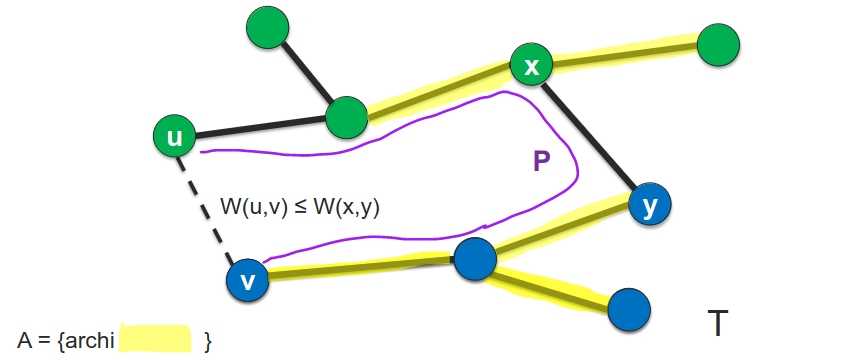
\includegraphics[width=80mm,scale=0.5]{arco_sicuro_dim_mst.png}
\end{center}
Il peso $W(u,v)$ è sicuramente $\leq$ rispetto al peso $W(x,y)$.\\
Sostituisco $(x,y)$, con $(u,v)$ e inserisco quindi l'arco $(u,v)$ all'interno
del grafo e noto che il grafo resta comunque un albero, vedo che resta un MST dato
che non ci sono cicli, ottengo quindi $T'$ con $W(T') \leq W(T)$.\\
\begin{center}
    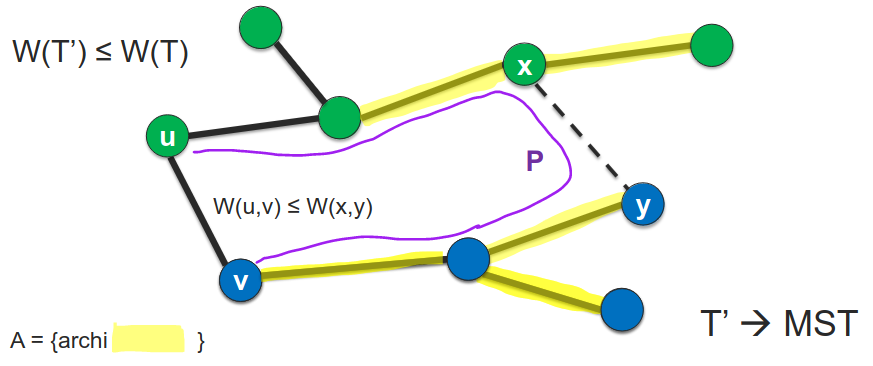
\includegraphics[width=80mm,scale=0.5]{arco_sicuro_dim_mst_2.png}
\end{center}
Per ipotesi, $A \subseteq T$ non contiene $(u,v)$ e $(x,y)$ e per costruzione $T'$ 
non contiene $(x,y)$.\\
$\implies A \subseteq T'$\\
$A \cup \{(u,v)\} \subseteq T'$
